\appendix
\chapter{Standard Libraries}
\section{Material Libraries}
\subsection{PCB Substrate Material Library}
Common substrate materials:
\begin{itemize}
\item FR4 -- Standard glass-reinforced epoxy laminate
\item Rogers -- High-frequency laminates
\item Metal-core -- Aluminum or copper core substrates
\end{itemize}

\subsection{PCB Conductor Material Library}
\begin{itemize}
\item Copper -- Standard conductor (specified in oz/ft$^2$)
\end{itemize}

\subsection{PCB Surface-finish Material Library}
\begin{itemize}
\item HASL -- Hot Air Solder Leveling
\item ENIG -- Electroless Nickel Immersion Gold
\item OSP -- Organic Solderability Preservative
\end{itemize}

\section{Basic Model Libraries}
\subsection{Passive Component Model Library}
\begin{itemize}
\item R -- Resistor (parameters: R, P, type)
\item C -- Capacitor
\item L -- Inductor
\end{itemize}

\subsection{Active Component Model Library}
\begin{itemize}
\item MOSFET -- MOSFET transistor
\item Diode -- Standard diode
\item BJT -- Bipolar junction transistor
\end{itemize}

\subsection{Integrated Circuit Component Model Library}
\begin{itemize}
\item opamp -- Operational amplifier
\item Additional models in external libraries
\end{itemize}

\subsection{Board Hardware Component Model Library}
\begin{itemize}
\item Connectors
\item Mounting holes
\end{itemize}

\section{Additional Language Libraries}
EDADSL can be extended with custom libraries containing component models, footprints, and constraint templates. Libraries follow the standard library organization.

\section{Footprint Libraries}
Footprints follow KiCad library naming conventions:
\begin{verbatim}
<Library>:<Footprint>

Examples:
Resistor_THT:R_Axial_DIN0309_L9.0mm_D3.2mm_P12.70mm_Horizontal
Package_TO_SOT_THT:TO-247-3_Horizontal_TabUp
Package_DIP:DIP-8_W7.62mm
\end{verbatim}


\chapter{Examples}
\section{LED Circuit}
\subsection{Intent}
A simple LED current-limiting circuit.

\subsection{EDADSL Code}
\begin{verbatim}
start

elec.part "R1": R(R=330, P=0.25); 
    des="330 ohm resistor"; 
    fp="Resistor_THT:R_Axial_DIN0309"
elec.part "D1": LED(color="red"); 
    des="Red LED"; 
    fp="LED_THT:LED_D3.0mm"

elec.net "Vcc"
elec.net "Gnd"

elec.connect Vcc R1[1]
elec.connect R1[2] D1[a]
elec.connect D1[c] Gnd

halt
\end{verbatim}

\subsection{Explanation}
The circuit connects a 330$\Omega$ resistor in series with an LED between Vcc and Gnd. The resistor limits current to approximately 10mA (assuming 5V supply and 2V LED forward voltage).

\section{Arithmetic and Type Coercion}
\subsection{Intent}
Demonstrate basic arithmetic, variable declarations, and implicit type promotion from int to real to complex.

\subsection{EDADSL Code}
\begin{verbatim}
start

$a [int]= 10
$b [real]= 3.14
$c [complex]= 2 + 3i

$sum t= $a + $b           #c# 13.14 (int + real -> real)
$prod t= $a * $c          #c# 20 + 30i (int * complex -> complex)
$hyp t= f.log.sqrt($a^2 + $b^2) #c# ~10.49 (real)
$ang t= f.cplx.angle($c)          #c# ~0.9828 rad (real)

f.util.print(f.str.str("a + b = ", $sum))
f.util.print(f.str.str("a * c = ", $prod))
f.util.print(f.str.str("hypotenuse = ", $hyp))
f.util.print(f.str.str("angle = ", $ang))

halt
\end{verbatim}

\subsection{Explanation}
Variables are declared with explicit types. Arithmetic operations implicitly promote to the wider type: int + real yields real, int + complex yields complex. The \texttt{f.cplx.angle} function returns the argument (phase) of a complex number in radians.

\section{Conditionals and Classification}
\subsection{Intent}
Use nested \texttt{if}/\texttt{else} to classify a resistor value into standard E-series ranges.

\subsection{EDADSL Code}
\begin{verbatim}
start

$value [real]= 4.7e3

$series [string]= ""
if $value < 1e3 ::{
    $series = "E12 or below"
} else ::{
    if $value < 100e3 ::{
        $series = "E24 common"
    } else ::{
        $series = "High value"
    }
}

$tolerance [string]= ""
if $value == 1.0e3 ::{
    $tolerance = "tight"
} else ::{
    if $value == 4.7e3 ::{
        $tolerance = "standard"
    } else ::{
        $tolerance = "check datasheet"
    }
}

f.util.print(f.str.str($value, " ohms: ", $series, ", ", $tolerance))

halt
\end{verbatim}

\subsection{Explanation}
The \texttt{if}/\texttt{otherwise}/\texttt{else} chain classifies the resistor into ranges. Use \texttt{otherwise} for else-if conditions. For cleaner multi-branch logic, use the \texttt{cases} statement. The expected output is \texttt{4700.0 ohms: E24 common, standard}.

\section{Lambdas and Higher-Order Functions}
\subsection{Intent}
Use lambda expressions with \texttt{f.util.map}, \texttt{f.util.filter}, and \texttt{f.util.reduce} to process a list of resistor values.

\subsection{EDADSL Code}
\begin{verbatim}
start

$resistors [list]= [100, 220, 330,
    470, 1e3, 2.2e3, 4.7e3, 10e3]

# Compute power dissipation at 5V
$powers [list]= f.util.map($resistors,
    L::($r [real]) -> { (5.0^2) / $r })
f.util.print(f.str.str("Powers: ", $powers))

# Filter to only resistors under 1k
$small [list]= f.util.filter($resistors,
    L::($r [real]) -> { $r < 1000 })
f.util.print(f.str.str("Under 1k: ", $small))

# Sum all power dissipation
$total_power [real]= f.util.reduce($powers,
    L::($acc [real], $p [real]) -> { $acc + $p },
    0.0)
f.util.print(f.str.str("Total power: ", $total_power, " W"))

# Sort resistors ascending
$sorted [list]= f.util.sort($resistors,
    L::($a [real], $b [real]) -> { $a - $b })
f.util.print(f.str.str("Sorted: ", $sorted))

halt
\end{verbatim}

\subsection{Explanation}
Lambdas are declared with \texttt{L::} prefix, typed parameters, and \texttt->\{\} body. \texttt{f.util.map} applies a function to each element, \texttt{f.util.filter} selects elements satisfying a predicate, and \texttt{f.util.reduce} folds the list with an accumulator. The sort comparator returns negative if the first argument should come first.

\section{Complex Arithmetic and FFT}
\subsection{Intent}
Perform complex arithmetic, generate a signal, and compute its frequency spectrum using FFT.

\subsection{EDADSL Code}
\begin{verbatim}
start

# Complex arithmetic
$z1 [complex]= 3 + 4i
$z2 [complex]= 1 - 2i

$sum     t= $z1 + $z2         # 4 + 2i
$product t= $z1 * $z2         # 11 - 2i
$mag     t= f.math.abs($z1)         # 5.0
$conj_z  t= f.cplx.conj($z2)        # 1 + 2i

f.util.print(f.str.str("|z1| = ", $mag))
f.util.print(f.str.str("z1 * z2 = ", $product))
f.util.print(f.str.str("conj(z2) = ", $conj_z))

# Generate a 256-point signal: 50Hz + 120Hz
$N [int]= 256
$fs [real]= 1000.0
$t [list]= [0:1:$N - 1]
$signal [list]= f.util.map($t,
    L::($n [int]) -> { f.trig.sin(2 * c.math.pi * 50
        * $n / $fs)
        + 0.5 * f.trig.sin(2 * c.math.pi * 120
        * $n / $fs) })

# Compute FFT and extract magnitudes
$spectrum [list]= f.ee.fft($signal)
$mags [list]= f.util.map($spectrum,
    L::($z [complex]) -> { f.math.abs($z) })

# Find the dominant frequency
$max_mag [real]= f.math.max($mags)
$peak_index [int]= f.stat.argmax($mags)
$freq [real]= ($peak_index * $fs) / $N

f.util.print(f.str.str("Dominant frequency: ", $freq, " Hz"))
f.util.print(f.str.str("Magnitude: ", $max_mag))

halt
\end{verbatim}

\subsection{Explanation}
Complex numbers support all arithmetic operators. The \texttt{f.ee.fft} function returns a list of complex values; \texttt{f.util.map} with \texttt{f.math.abs} extracts magnitudes. The dominant frequency is recovered by finding the index of the peak magnitude and scaling by $f_s / N$. The expected dominant frequency is 50 Hz.

\section{Ndarray Matrix Operations}
\subsection{Intent}
Use tensor syntax and matrix operators to solve a system of linear equations.

\subsection{EDADSL Code}
\begin{verbatim}
start

# Solve A * x = b where:
#   A = [[2, 1], [5, 7]]
#   b = [11, 13]
$A [tensor]= |[[2, 1], [5, 7]]
$b [tensor]= |[11, 13]

# Compute inverse and solve
$A_inv [tensor]= f.linalg.inv($A)
$x [tensor]= $A_inv .* $b

f.util.print(f.str.str("Solution x = ", $x))

# Verify: A .* x should equal b
$check [tensor]= $A .* $x
f.util.print(f.str.str("Verification A .* x = ", $check))

# Matrix properties
f.util.print(f.str.str("det(A) = ", f.linalg.det($A)))
f.util.print(f.str.str("rank(A) = ", f.linalg.rank($A)))

halt
\end{verbatim}

\subsection{Explanation}
Tensors are explicitly typed with \texttt{[tensor]} or pipe literal syntax. The \texttt{.*} operator performs matrix multiplication, and \texttt{f.linalg.inv} computes the matrix inverse. Functions \texttt{f.linalg.det} and \texttt{f.linalg.rank} return the determinant and rank respectively. The expected solution is $x = [6.2, -1.4]$.

\section{Closures and Lambdas}
\subsection{Intent}
Demonstrate lambdas capturing outer variables and lambda composition for filtering and mapping.

\subsection{EDADSL Code}
\begin{verbatim}
start

$resistors [list]= [100, 330, 1e3, 2.2e3, 4.7e3, 10e3]

# Filter: keep resistors above 1k (captures $threshold)
$threshold [real]= 1000
$high [list]= f.util.filter($resistors,
    L::($v [real]) -> { $v > $threshold })
f.util.print(f.str.str("Above 1k: ", $high))

# Filter: keep resistors above 4.7k
$threshold = 4700
$vhigh [list]= f.util.filter($resistors,
    L::($v [real]) -> { $v > $threshold })
f.util.print(f.str.str("Above 4.7k: ", $vhigh))

# Element-wise add scalar to each list element
$offset [int]= 10
$shifted [list]= f.util.map([10, 20, 30],
    L::($i [int]) -> { $i + $offset })
f.util.print(f.str.str("Shifted: ", $shifted))

halt
\end{verbatim}

\subsection{Explanation}
Lambdas capture variables from the enclosing scope. Here \texttt{\$threshold} is captured by reference: reassigning it before calling \texttt{f.util.filter} changes which values pass the filter. The \texttt{f.util.map} lambda captures \texttt{\$offset} to add a constant to each element.

\section{Design-Rule-Driven Component Placement}
\subsection{Intent}
Declare components with parametric constraints and let the solver handle placement.

\subsection{EDADSL Code}
\begin{verbatim}
start

elec.part "U1": opamp(type="generic", GBP=1e6, slew=5)
    ; des="Generic op-amp"
    ; fp="Package_DIP:DIP-8_W7.62mm"

elec.part "Rf": R(R=10e3, P=0.125, tol=1)
    ; des="Feedback resistor"
    ; fp="Resistor_THT:R_Axial_DIN0309"

elec.part "Rin": R(R=1e3, P=0.125, tol=1)
    ; des="Input resistor"
    ; fp="Resistor_THT:R_Axial_DIN0309"

elec.part "C1": C(C=100e-12, V=50)
    ; des="Compensation capacitor"
    ; fp="Capacitor_THT:C_Axial_DIN0207"

elec.net "Input"
elec.net "Output"
elec.net "Vcc"
elec.net "Gnd"

elec.connect Input Rin[1]
elec.connect Rin[2] U1[2]      # inverting input
elec.connect Rf[1] U1[2]
elec.connect Rf[2] U1[1]       # output
elec.connect C1[1] U1[2]
elec.connect C1[2] U1[1]
elec.connect Output U1[1]
elec.connect U1[4] Vcc
elec.connect U1[7] Gnd

# Constraint: keep feedback path short
phys.prox {Rf} {U1} max=15m -imp

halt
\end{verbatim}

\subsection{Explanation}
Components are declared with parametric models and footprint assignments using \texttt{;} separators. The \texttt{phys.prox} keyword specifies a physical layout constraint that the placement solver must satisfy. This example inverts the op-amp with gain $G = -R_f / R_{in} = -10$ and includes compensation.

\section{Signal Processing Pipeline}
\subsection{Intent}
Build a complete signal processing pipeline: generate, filter, transform, and analyze.

\subsection{EDADSL Code}
\begin{verbatim}
start

# Step 1: Generate a noisy 100Hz signal
$N [int]= 512
$fs [real]= 1000.0
$t [list]= [0:1:$N - 1]
$clean [list]= f.util.map($t,
    L::($n [int]) -> { f.trig.sin(2 * c.math.pi
        * 100 * $n / $fs) })

# Step 2: Add noise (simple LCG pseudo-random)
$noise [list]= f.util.map($t,
    L::($n [int]) -> { 0.3 * f.trig.sin(2 * c.math.pi
        * 7 * $n) })
$noisy [list]= f.util.map($t,
    L::($i [int]) -> { $clean[$i] + $noise[$i] })

# Step 3: Compute FFT of noisy signal
$spectrum [list]= f.ee.fft($noisy)
$mags [list]= f.util.map($spectrum,
    L::($z [complex]) -> { f.math.abs($z) })

# Step 4: Find peak frequency
$peak_idx [int]= f.stat.argmax($mags)
$peak_freq [real]= ($peak_idx * $fs) / $N
f.util.print(f.str.str("Detected frequency: ", $peak_freq, " Hz"))

# Step 5: Compute signal statistics
$sig_rms [real]= f.stat.rms($noisy)
$sig_peak [real]= f.stat.peak($noisy)
f.util.print(f.str.str("RMS: ", $sig_rms, ", Peak: ", $sig_peak))

# Step 6: Build magnitude spectrum pairs
$bin_width [real]= $fs / $N
$spec_pairs [list]= []
for $i E [0:1:$N / 2 - 1] ::{
    $freq_val [real]= $i * $bin_width
    $mag_val [real]= $mags[$i]
    $spec_pairs = $spec_pairs
        + [[$freq_val, $mag_val]]
}

f.util.print(f.str.str("Spectrum bins (first 5): ",
    $spec_pairs[0:5]))

halt
\end{verbatim}

\subsection{Explanation}
This example chains together multiple language features: \texttt{f.util.map} for list comprehensions, complex FFT, higher-order functions for magnitude extraction, signal statistics (\texttt{f.stat.rms}, \texttt{f.stat.peak}), and list slicing. The pipeline demonstrates a realistic signal analysis workflow from raw data through frequency-domain representation.

\chapter{Diagrams}

\section{Execution-phase Diagram}
The following diagram shows the execution phases of an EDADSL program, from source code through constraint solving to final output.

\begin{center}
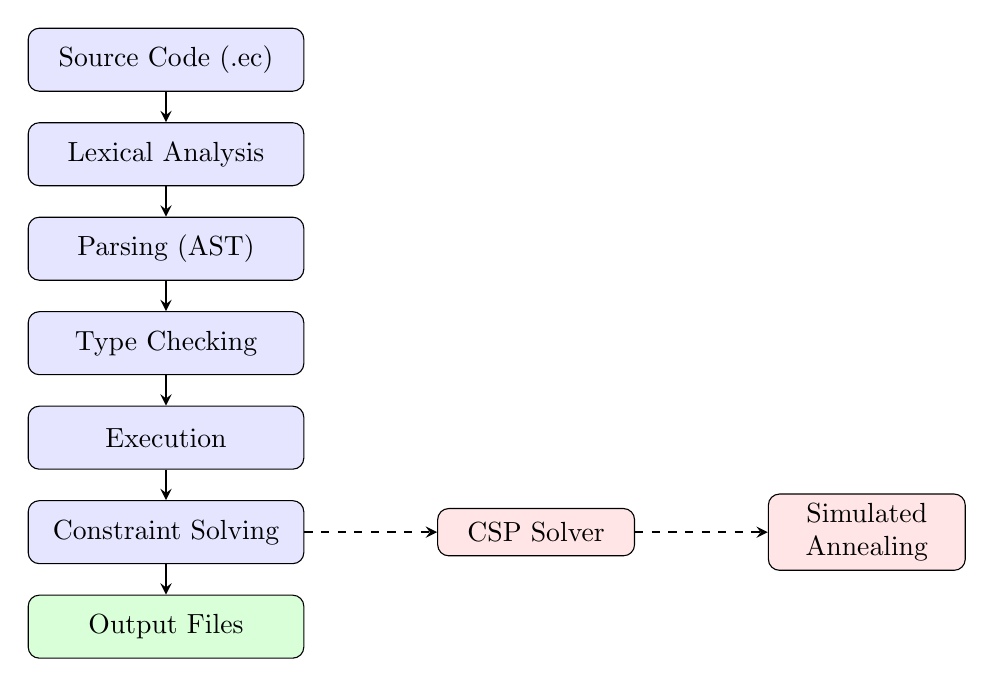
\begin{tikzpicture}[
    >=stealth,
    node distance=1.2cm,
    every node/.style={draw, rectangle, rounded corners, minimum width=3.5cm, minimum height=0.8cm, align=center, fill=blue!10},
    arrow/.style={->, thick, draw=black}
]
  \node (src) {Source Code (.ec)};
  \node (lex) [below of=src] {Lexical Analysis};
  \node (parse) [below of=lex] {Parsing (AST)};
  \node (check) [below of=parse] {Type Checking};
  \node (exec) [below of=check] {Execution};
  \node (solve) [below of=exec] {Constraint Solving};
  \node (output) [below of=solve, fill=green!15] {Output Files};

  \draw[arrow] (src) -- (lex);
  \draw[arrow] (lex) -- (parse);
  \draw[arrow] (parse) -- (check);
  \draw[arrow] (check) -- (exec);
  \draw[arrow] (exec) -- (solve);
  \draw[arrow] (solve) -- (output);

  % Side nodes for constraint solving
  \node[draw, rectangle, rounded corners, minimum width=2.5cm, minimum height=0.6cm, align=center, fill=red!10, right of=solve, xshift=3.5cm] (csp) {CSP Solver};
  \node[draw, rectangle, rounded corners, minimum width=2.5cm, minimum height=0.6cm, align=center, fill=red!10, right of=csp, xshift=3cm] (sa) {Simulated\\Annealing};

  \draw[arrow, dashed] (solve) -- (csp);
  \draw[arrow, dashed] (csp) -- (sa);
\end{tikzpicture}
\end{center}

\vspace{5mm}
\textbf{Phase Descriptions:}
\begin{itemize}
\item \textbf{Lexical Analysis} -- Tokenizes the source file into keywords, identifiers, literals, and operators.
\item \textbf{Parsing} -- Builds an Abstract Syntax Tree (AST) from the token stream.
\item \textbf{Type Checking} -- Validates types, performs implicit promotions, and resolves overloads.
\item \textbf{Execution} -- Evaluates expressions, executes control flow, and evaluates functions. Components and nets are registered.
\item \textbf{Constraint Solving} -- Physical constraints are solved using CSP propagation and simulated annealing to determine optimal placement and routing.
\item \textbf{Output Files} -- Generates manufacturing files (Gerbers, drill files, BOM, netlists).
\end{itemize}

\section{Type Hierarchy Diagram}
The following diagram shows the EDADSL type hierarchy, including numeric promotion, collection types, and their relationships.

\begin{center}
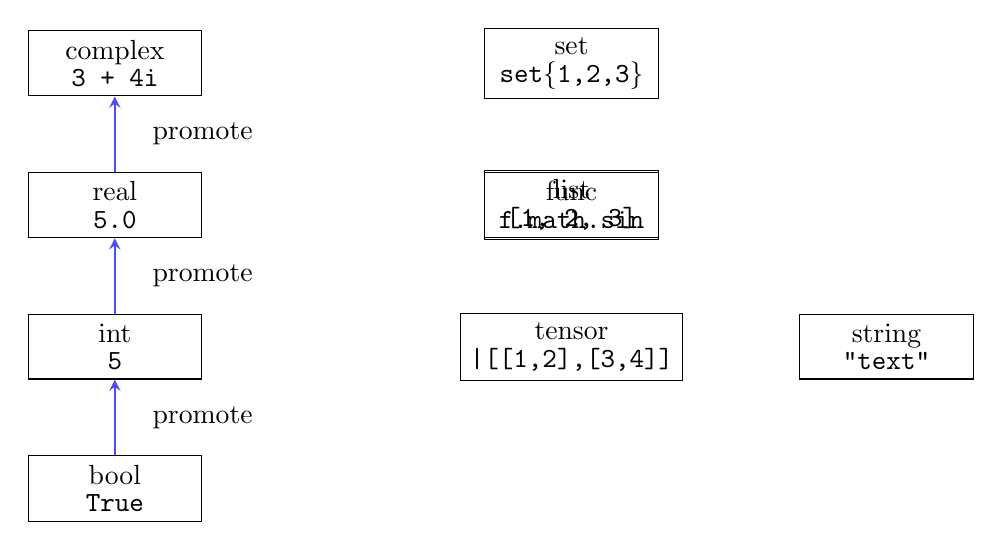
\begin{tikzpicture}[
    >=stealth,
    node distance=1.8cm,
    every node/.style={draw, rectangle, minimum width=2.2cm, minimum height=0.8cm, align=center},
    promote/.style={->, thick, draw=blue!70}
]
  % Numeric hierarchy
  \node (bool) {bool\\[-2pt]\texttt{True}};
  \node (int) [above of=bool] {int\\[-2pt]\texttt{5}};
  \node (real) [above of=int] {real\\[-2pt]\texttt{5.0}};
  \node (complex) [above of=real] {complex\\[-2pt]\texttt{3 + 4i}};

  \draw[promote] (bool) -- node[right, draw=none] {promote} (int);
  \draw[promote] (int) -- node[right, draw=none] {promote} (real);
  \draw[promote] (real) -- node[right, draw=none] {promote} (complex);

  % Collection types
  \node (string) [right of=int, xshift=8cm] {string\\[-2pt]\texttt{"text"}};
  \node (list) [right of=real, xshift=4cm] {list\\[-2pt]\texttt{[1, 2, 3]}};
  \node (set) [right of=complex, xshift=4cm] {set\\[-2pt]\texttt{set\{1,2,3\}}};
  \node (tensor) [below of=list] {tensor\\[-2pt]\texttt{|[[1,2],[3,4]]}};
  \node (func) [below of=set] {func\\[-2pt]\texttt{f.math.sin}};
\end{tikzpicture}
\end{center}

\vspace{5mm}
\textbf{Key Relationships:}
\begin{itemize}
\item Numeric types promote automatically: \texttt{bool} $\rightarrow$ \texttt{int} $\rightarrow$ \texttt{real} $\rightarrow$ \texttt{complex}
\item A \texttt{tensor} is a \texttt{list} that is rectangular and all-numeric; explicitly typed with \texttt{[tensor]} or pipe literal \texttt{|[...]}
\item \texttt{list} element types are polymorphic; \texttt{tensor} elements are restricted to \texttt{bool}, \texttt{int}, \texttt{real}, or \texttt{complex}
\item \texttt{set} is unordered and unique; \texttt{list} is ordered and allows duplicates
\item \texttt{func} values are callable; they can be built-in references, user-defined references, or lambdas
\end{itemize}

\section{Operator Precedence Diagram}
The following diagram visualizes operator precedence from highest (top) to lowest (bottom).

\begin{center}
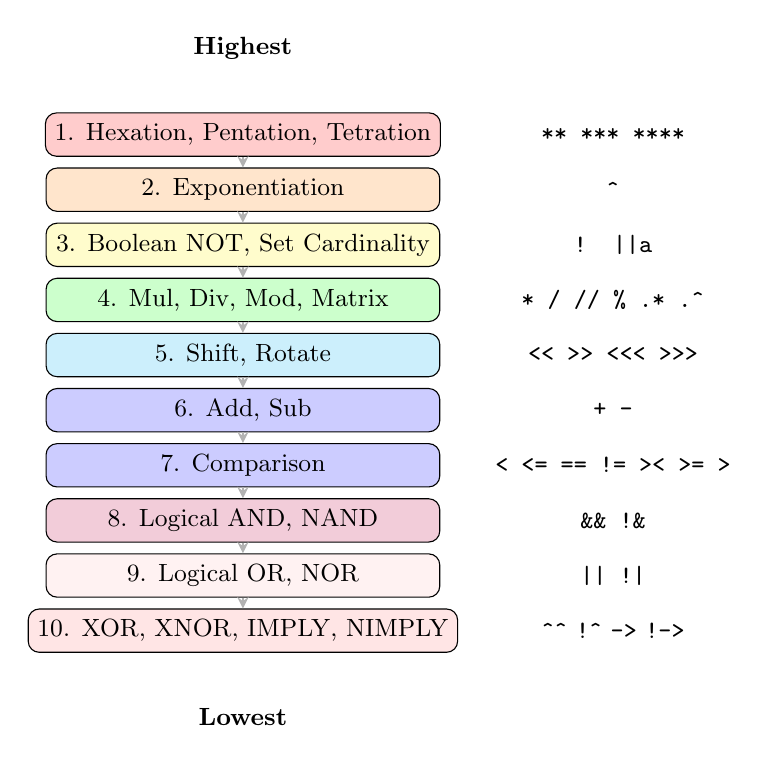
\begin{tikzpicture}[
    >=stealth,
    node distance=0.7cm,
    level/.style={draw, rectangle, rounded corners, minimum width=5cm, minimum height=0.55cm, align=center, font=\small},
    arrow/.style={->, thick, draw=gray!60}
]
  \node[level, fill=red!20]    (p0) {1. Hexation, Pentation, Tetration};
  \node[level, fill=orange!20] (p1) [below of=p0] {2. Exponentiation};
  \node[level, fill=yellow!20] (p2) [below of=p1] {3. Boolean NOT, Set Cardinality};
  \node[level, fill=green!20] (p3) [below of=p2] {4. Mul, Div, Mod, Matrix};
  \node[level, fill=cyan!20]  (p4) [below of=p3] {5. Shift, Rotate};
  \node[level, fill=blue!20]  (p5) [below of=p4] {6. Add, Sub};
  \node[level, fill=blue!20]  (p6) [below of=p5] {7. Comparison};
  \node[level, fill=purple!20] (p7) [below of=p6] {8. Logical AND, NAND};
  \node[level, fill=pink!20]  (p8) [below of=p7] {9. Logical OR, NOR};
  \node[level, fill=red!10]  (p9) [below of=p8] {10. XOR, XNOR, IMPLY, NIMPLY};

  \draw[arrow] (p0) -- (p1);
  \draw[arrow] (p1) -- (p2);
  \draw[arrow] (p2) -- (p3);
  \draw[arrow] (p3) -- (p4);
  \draw[arrow] (p4) -- (p5);
  \draw[arrow] (p5) -- (p6);
  \draw[arrow] (p6) -- (p7);
  \draw[arrow] (p7) -- (p8);
  \draw[arrow] (p8) -- (p9);

  % Annotations on the right
  \node[draw=none, font=\small, right of=p0, xshift=4cm] {\texttt{** *** ****}};
  \node[draw=none, font=\small, right of=p1, xshift=4cm] {\texttt{\^{}}};
  \node[draw=none, font=\small, right of=p2, xshift=4cm] {\texttt{! ||a}};
  \node[draw=none, font=\small, right of=p3, xshift=4cm] {\texttt{* / // \% .* .\^{}}};
  \node[draw=none, font=\small, right of=p4, xshift=4cm] {\texttt{<< >> <<< >>>}};
  \node[draw=none, font=\small, right of=p5, xshift=4cm] {\texttt{+ -}};
  \node[draw=none, font=\small, right of=p6, xshift=4cm] {\texttt{< <= == != >< >= >}};
  \node[draw=none, font=\small, right of=p7, xshift=4cm] {\texttt{\&\& !\&}};
  \node[draw=none, font=\small, right of=p8, xshift=4cm] {\texttt{|| !|}};
  \node[draw=none, font=\small, right of=p9, xshift=4cm] {\texttt{\^{}}\texttt{\^{}} \texttt{!}\texttt{\^{}} \texttt{->} \texttt{!->}};

  % Label
  \node[draw=none, font=\small\bfseries, above of=p0, yshift=0.4cm] {Highest};
  \node[draw=none, font=\small\bfseries, below of=p9, yshift=-0.4cm] {Lowest};
\end{tikzpicture}
\end{center}

\vspace{5mm}
\textbf{Precedence Table:}
\begin{enumerate}
\item Hexation (\texttt{****}), Pentation (\texttt{***}), Tetration (\texttt{**}) -- right-associative
\item Exponentiation (\texttt{\^{}}) -- right-associative
\item Boolean negation (\texttt{!}), Set cardinality (\texttt{||a})
\item Multiplication (\texttt{*}), Division (\texttt{/}), Floor Division (\texttt{//}), Modulo (\texttt{\%}), Matrix (\texttt{.* .\^{}})
\item Shift (\texttt{<< >>}), Rotate (\texttt{<<<[w] >>>[w]})
\item Addition (\texttt{+}), Subtraction (\texttt{-})
\item Comparison (\texttt{< <= == != >< >= >})
\item Logical AND (\texttt{\&\&}), NAND (\texttt{!\&})
\item Logical OR (\texttt{||}), NOR (\texttt{!|})
\item XOR (\texttt{\^{}}\texttt{\^{}}), XNOR (\texttt{!}\texttt{\^{}}), IMPLY (\texttt{->}), NIMPLY (\texttt{!->})
\end{enumerate}

\section{Example Circuit: LED Current-Limiting}
The following diagram shows the LED circuit from Appendix B alongside its EDADSL code.

\begin{center}
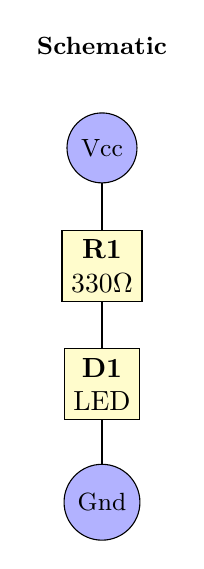
\begin{tikzpicture}[
    >=stealth,
    component/.style={draw, rectangle, minimum width=1.5cm, minimum height=0.6cm, align=center, fill=yellow!20},
    net/.style={draw, circle, minimum size=0.4cm, fill=blue!30},
    wire/.style={thick}
]
  % Circuit schematic
  \node[net] (vcc) at (0,3) {\small Vcc};
  \node[component, minimum width=0.8cm] (r1) at (0,1.5) {\textbf{R1}\\330$\Omega$};
  \node[component, minimum width=0.8cm] (d1) at (0,0) {\textbf{D1}\\LED};
  \node[net] (gnd) at (0,-1.5) {\small Gnd};

  \draw[wire] (vcc) -- (r1);
  \draw[wire] (r1) -- (d1);
  \draw[wire] (d1) -- (gnd);

  % Labels
  \node[above of=vcc, yshift=0.3cm, draw=none, font=\small\bfseries] {Schematic};
\end{tikzpicture}
\end{center}

\textbf{EDADSL Code:}
\begin{verbatim}
elec.part "R1": R(R=330)
    des="330 ohm"
    fp="Resistor_THT:R_Axial"
elec.part "D1": LED(color="red")
    des="Red LED"
    fp="LED_THT:LED_D3.0mm"

elec.net "Vcc"
elec.net "Gnd"

elec.connect Vcc R1[1]
elec.connect R1[2] D1[a]
elec.connect D1[c] Gnd
\end{verbatim}

\vspace{5mm}
\textbf{Circuit Description:} A 330$\Omega$ resistor (R1) limits current through a red LED (D1) between Vcc (5V) and Gnd. Expected current: $I = (5V - 2V) / 330\Omega \approx 9.1\text{mA}$.

\section{FFT Pipeline Diagram}
The following diagram shows the signal processing pipeline for FFT analysis.

\begin{center}
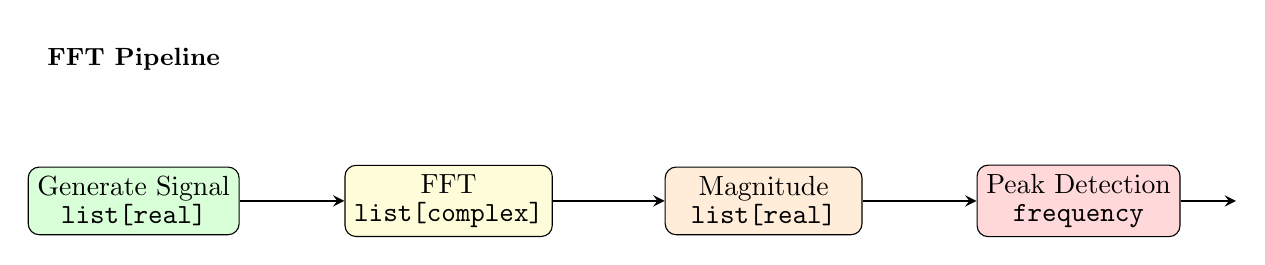
\begin{tikzpicture}[
    >=stealth,
    node distance=1.5cm,
    every node/.style={draw, rectangle, rounded corners, minimum width=2.5cm, minimum height=0.8cm, align=center},
    arrow/.style={->, thick, draw=black}
]
  \node[fill=green!15] (gen) {Generate Signal\\[-2pt]\texttt{list[real]}};
  \node[fill=yellow!15, right of=gen, xshift=2.5cm] (fft) {FFT\\[-2pt]\texttt{list[complex]}};
  \node[fill=orange!15, right of=fft, xshift=2.5cm] (mag) {Magnitude\\[-2pt]\texttt{list[real]}};
  \node[fill=red!15, right of=mag, xshift=2.5cm] (peak) {Peak Detection\\[-2pt]\texttt{frequency}};

  \draw[arrow] (gen) -- (fft);
  \draw[arrow] (fft) -- (mag);
  \draw[arrow] (mag) -- (peak);
  \draw[arrow] (peak) -- ++(2,0);

  % Labels
  \node[above of=gen, yshift=0.3cm, draw=none, font=\small\bfseries] {FFT Pipeline};
\end{tikzpicture}
\end{center}

\textbf{EDADSL Code:}
\begin{verbatim}
$signal [list]= f.util.map([0:1:$N - 1],
    L::($n [int]) -> { f.trig.sin(2 * c.math.pi
        * 100 * $n / $fs) })
$spectrum [list]= f.ee.fft($signal)
    # list[complex]
$mags     [list]= f.util.map($spectrum,
    L::($z [complex]) -> { f.math.abs($z) })
    # list[real]
$peak_idx [int]= f.stat.argmax($mags)
$freq     [real]= ($peak_idx * $fs) / $N   # = 100 Hz
\end{verbatim}

\section{Ndarray Operations}
The following diagram visualizes key tensor operations: element-wise operations, matrix multiplication, and broadcasting.

\begin{center}
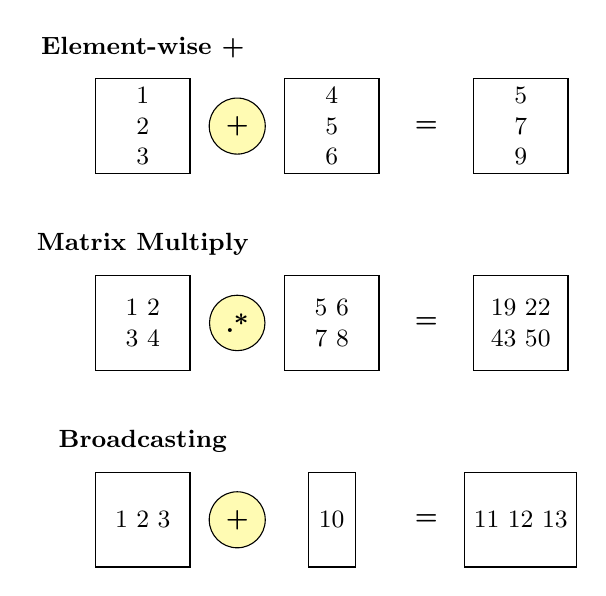
\begin{tikzpicture}[
    >=stealth,
    node distance=0.8cm,
    matrix/.style={draw, minimum width=1.2cm, minimum height=1.2cm, align=center, font=\small},
    op/.style={draw, circle, minimum size=0.6cm, fill=yellow!30, font=\small\bfseries}
]
  % Element-wise addition
  \node[draw=none, font=\small\bfseries] at (0, 2.5) {Element-wise +};
  \node[matrix] (a1) at (0, 1.5) {1\\2\\3};
  \node[op] (plus) at (1.2, 1.5) {+};
  \node[matrix] (b1) at (2.4, 1.5) {4\\5\\6};
  \node[draw=none, font=\small\bfseries] at (3.6, 1.5) {=};
  \node[matrix] (c1) at (4.8, 1.5) {5\\7\\9};

  % Matrix multiply
  \node[draw=none, font=\small\bfseries] at (0, 0) {Matrix Multiply};
  \node[matrix] (a2) at (0, -1) {1 2\\3 4};
  \node[op] (dot) at (1.2, -1) {.*};
  \node[matrix] (b2) at (2.4, -1) {5 6\\7 8};
  \node[draw=none, font=\small\bfseries] at (3.6, -1) {=};
  \node[matrix] (c2) at (4.8, -1) {19 22\\43 50};

  % Broadcasting
  \node[draw=none, font=\small\bfseries] at (0, -2.5) {Broadcasting};
  \node[matrix] (a3) at (0, -3.5) {1 2 3};
  \node[op] (plus3) at (1.2, -3.5) {+};
  \node[matrix, minimum width=0.6cm] (b3) at (2.4, -3.5) {10};
  \node[draw=none, font=\small\bfseries] at (3.6, -3.5) {=};
  \node[matrix] (c3) at (4.8, -3.5) {11 12 13};
\end{tikzpicture}
\end{center}

\textbf{EDADSL Code:}
\begin{verbatim}
$a [tensor]= |[1, 2, 3]
$b [tensor]= |[4, 5, 6]
$a + $b         #c# = |[5, 7, 9]
$m1 [tensor]= |[[1,2],[3,4]]
$m2 [tensor]= |[[5,6],[7,8]]
$m1 .* $m2      #c# = |[[19,22],[43,50]]
$a + 10         #c# = |[11, 12, 13]
\end{verbatim}

\vspace{5mm}
\textbf{Operations:}
\begin{itemize}
\item \textbf{Element-wise} -- Standard operators (\texttt{+ - * / \^{} }) applied element-by-element
\item \textbf{Matrix Multiply} -- \texttt{.*} computes matrix product (rows $\times$ columns)
\item \textbf{Broadcasting} -- Scalars are broadcast to match the tensor shape
\item \textbf{Transpose} -- \texttt{.T} flips rows and columns; \texttt{~.T} in-place
\end{itemize}

\section{Custom Model Definition and Usage}
\subsection{Intent}
Define a custom SiC MOSFET model with a kelvin source pin, then use it in a half-bridge circuit.

\subsection{EDADSL Code}
\begin{verbatim}
# Define custom SiC MOSFET model
elec.makemodel mosfet/C3M0016120K1:{
pins:
    g        -> 4; T = input
    s        -> 2; T = power
    d        -> 1; T = power
    kelvin_s -> 3; T = output

des = "1200 V, 125A, 16 mOhm, TO-247-4"
dts = "https://assets.wolfspeed.com/..."
fp  = "Package_TO_SOT_THT/TO-247-4_Vert"
}

# Use custom model in a half-bridge
elec.part "Q1": mosfet/C3M0016120K1();
    des="High-side SiC MOSFET";
    fp="Package_TO_SOT_THT/TO-247-4_Vert";
    show_ref=True; show_value=True

elec.part "Q2": mosfet/C3M0016120K1();
    des="Low-side SiC MOSFET";
    fp="Package_TO_SOT_THT/TO-247-4_Vert";
    show_ref=True; show_value=True

# Define nets
elec.net "Vbus" "hv"
elec.net "Vphase"
elec.net "Vgate_high"
elec.net "Vgate_low"
elec.net "Gnd"

# Gate drive
elec.connect Vgate_high Q1[g]
elec.connect Vgate_low  Q2[g]

# Half-bridge output
elec.connect Vphase Q1[d] Q2[d]

# Power rails
elec.connect Vbus Q1[s]
elec.connect Gnd  Q2[s]

# Kelvin connections for gate drive return
elec.connect Vgate_low Q1[kelvin_s]
elec.connect Gnd       Q2[kelvin_s]

# Unite into single physical package
phys.unite { Q1, Q2 }
\end{verbatim}

\subsection{Explanation}
The \texttt{elec.makemodel} keyword defines a new component model with named pins, pin types, and optional metadata. Pin types (\texttt{input}, \texttt{power}, \texttt{output}) classify the electrical role of each pin. The \texttt{des}, \texttt{dts}, and \texttt{fp} fields attach documentation and footprint information to the model.

When used in \texttt{elec.part}, the custom model is referenced by its full name (\texttt{mosfet/C3M0016120K1}). Per-component PCB text flags (\texttt{show\_ref}, \texttt{show\_value}) override the global defaults. The \texttt{phys.unite} statement merges Q1 and Q2 into a single physical package on the PCB.

